\section{Maturation}

Key papers: Abrusan 2013 \cite{abrusan_integration_2013}, Carvunis
\cite{carvunis_proto-genes_2012}

\subsection{Protein properties}
    \subsubsection{Rise in length} 

        I am suspicious of the length trend. It seems too perfect.  Since
        exon length is fairly constant across the strata, the increase in
        total length must be due to an increase in exon number. Exons can
        be shuffled about (how quickly? This is a vitally important thing
        to know), so the chance of one being homologous to something
        ancient increases with their count. So it could simply be that
        genes with more exons are more likely to be classified as ancient.
                
        Monotonic rise in orphan length ~6 fold: primates
        \cite{neme_phylogenetic_2013, toll-riera_origin_2009}, fish
        \cite{neme_phylogenetic_2013}, mice \cite{neme_phylogenetic_2013},
        Arabidopsis thaliana \cite{guo_gene_2013}, yeast
        \cite{carvunis_proto-genes_2012}

        De novo genes tend to be short: 69 mouse de novo genes (62-174), 6 rat
        de novo genes (70-208) \cite{murphy_novo_2012}.
        
        Lineage-specific genes are shorter than non-lineage-specific genes: in
        insects \cite{wissler_mechanisms_2013}.

        POFs all shorter too \cite{gollery_what_2006} 

        Interestingly, in \textit{Leishmania major} orphans are longer than
        non-orphans \cite{mukherjee_elucidating_2015}. I suspect this is
        partially due to the high GC content of \textit{L. major} (~60\%).

        \textbf{So where does all this new material in older genes come from?}
        It seems exon length stays roughly the same and new domains are added
        with time.

        Supported by Neme \cite{neme_phylogenetic_2013}, exon length stays
        roughly the same, so increase in length is due primarily to
        proliferation of exons.

        Heavily cited review of shuffling and duplication in maize
        \cite{morgante_gene_2005}

        Review of transposon stuff in flowering plants
        \cite{bennetzen_transposable_2005}. Describes how two newly discovered
        genes, Helitrons and Pack-MULEs, rearrange and fuse gene fragments,
        producing novel chimeric genes. However, while recent chimeras may be
        expressed, says none of these have proven to be retained. Plants have much
        more mobile genomes. Vast seas of repetative elements, decaying tansposons,
        active transposons with hackable promoters.

        Orphan domains are more likely to be disordered and spread more rapidly
        than established domains \cite{moore_dynamics_2011}.

        Moore has written a great many papers on the dynamics of protein
        domains \cite{moore_arrangements_2008, moore_dynamics_2011,
        moore_quantification_2013}

    \subsubsection{Increase in amino acid deviation from random}

        Correlation between orphan age and composition bias in 47
        prokaryotic genomes \cite{yomtovian_composition_2010}. As orphans
        age, their composition shifts gradually from one similar to random
        genomic material to compositions typical of mature proteins.

        In yeast, D, E, and C all differ very significantly between orphans
        and mature. Orphans resemble random
        \cite{carvunis_proto-genes_2012}

    \subsubsection{Increase in number of domains}

        Neme reports an increase, but it isn't a steady one. There is
        nothing in the top few strata then suddenly very many, bouncy and
        erratic between strata \cite{neme_phylogenetic_2013}.

    \subsubsection{Alpha helices percentage}

        In yeast, steady at ~40\%, regardless of ps
        \cite{abrusan_integration_2013} 

        \begin{figure}[h!] \centering
            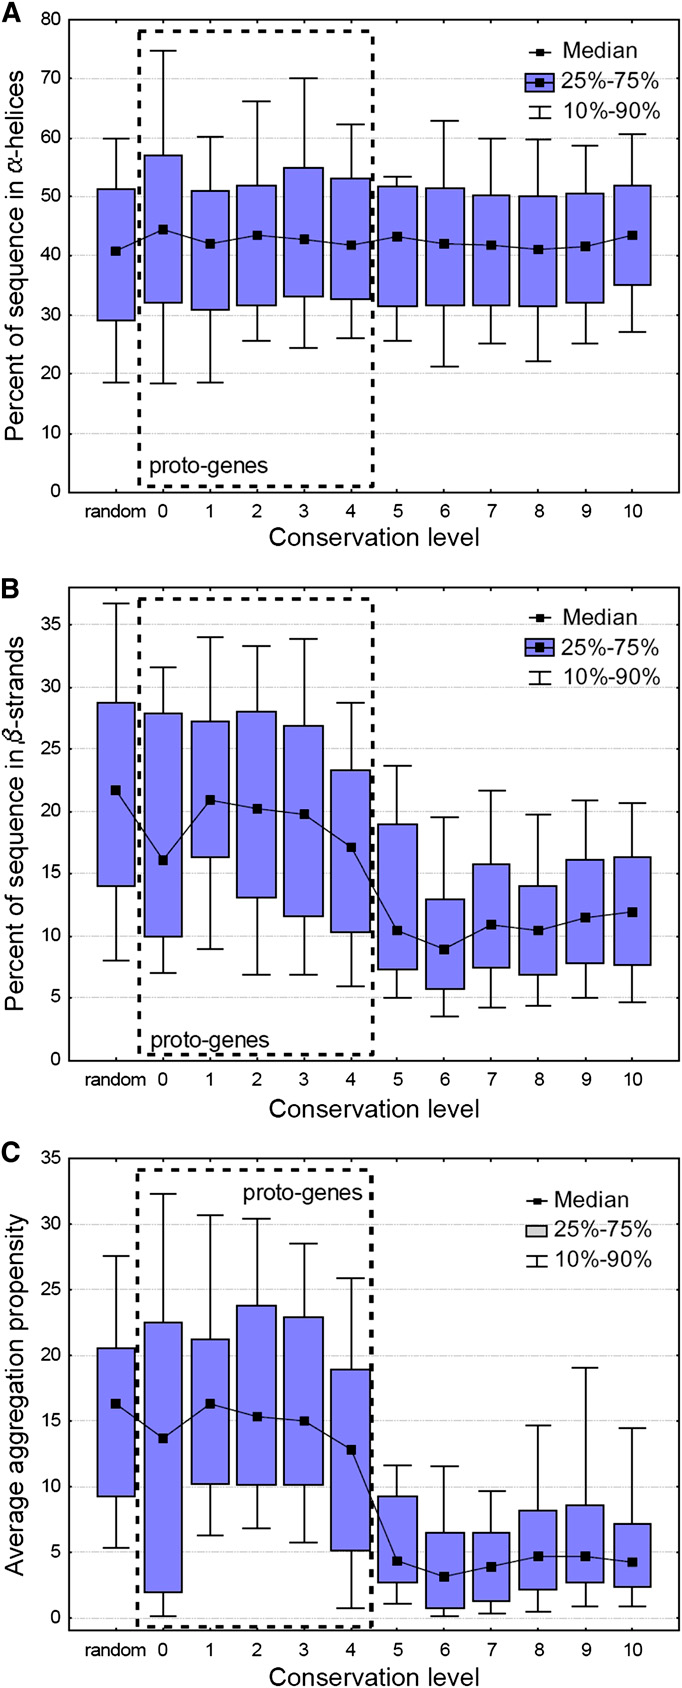
\includegraphics[scale=0.3]{abrusan-fig4} \caption{Abrusan
            (2013) structural trends} \end{figure} \FloatBarrier


    \subsubsection{Beta sheet percentage}

        In yeast, ~20\% in random sequence and protogenes, falls to 10\% in
        lower strata (extremely significant $pval << 0.001$)
        \cite{abrusan_integration_2013}. Perhaps due to selective pressure
        against aggregation propensity, which is high in b-sheets.

    \subsubsection{Aggregation propensity}

        Falls similarly to b-sheets, highly dependent
        \cite{abrusan_integration_2013}.

        While it is tempting to predict this is driven by evolutionary
        pressure against the toxicity of protein aggregates, there is not
        support for this. The protogenes Abrusan studies do not appear to
        be under strong selection \cite{carvunis_proto-genes_2012}. Abrusan
        proposes that proto-genes with high $\beta$ content tend to be
        de-genified. He finds there is high turnover in protogene
        populations.

    \subsubsection{Intrinsic disorder}

        Proteins secondary structure is more robust than intrinsic disorder
        \cite{schaefer_protein_2010}

        The disorder trend is quite interesting, it appears that disorder
        actually increases in the transition from non-genic to young
        orphan. Continues to increase steadily across strata, reaches a
        peak, and then falls \cite{carvunis_proto-genes_2012}.

        POFs ($~$60\% of which are clade-restricted) are \textbf{more}
        disordered than PDFs \cite[review]{gollery_pofs:_2007} and
        originally \cite{gollery_what_2006}.

    \subsubsection{Robusteness to mutation}

        Protogenes' secondary structure is more prone to change with
        mutations.  Older genes become more robust to mutation
        \cite{abrusan_integration_2013}. Clear increase across the strata,
        seems continuous increase, but is erratic. $\beta$ sheets are less
        robust under random mutation that $\alpha$ helices. But Abrusan
        shows that the trend is not an artefact of the higher $\beta$
        content of younger genes, being conserved even when $\beta$ sheets
        are removed from the analysis.

        Robustness of protein structure is important for evolutionary
        innovation \cite{bloom_structural_2006, bloom_protein_2006,
        bloom_evolution_2007}.

        \begin{figure}[h!] \centering
            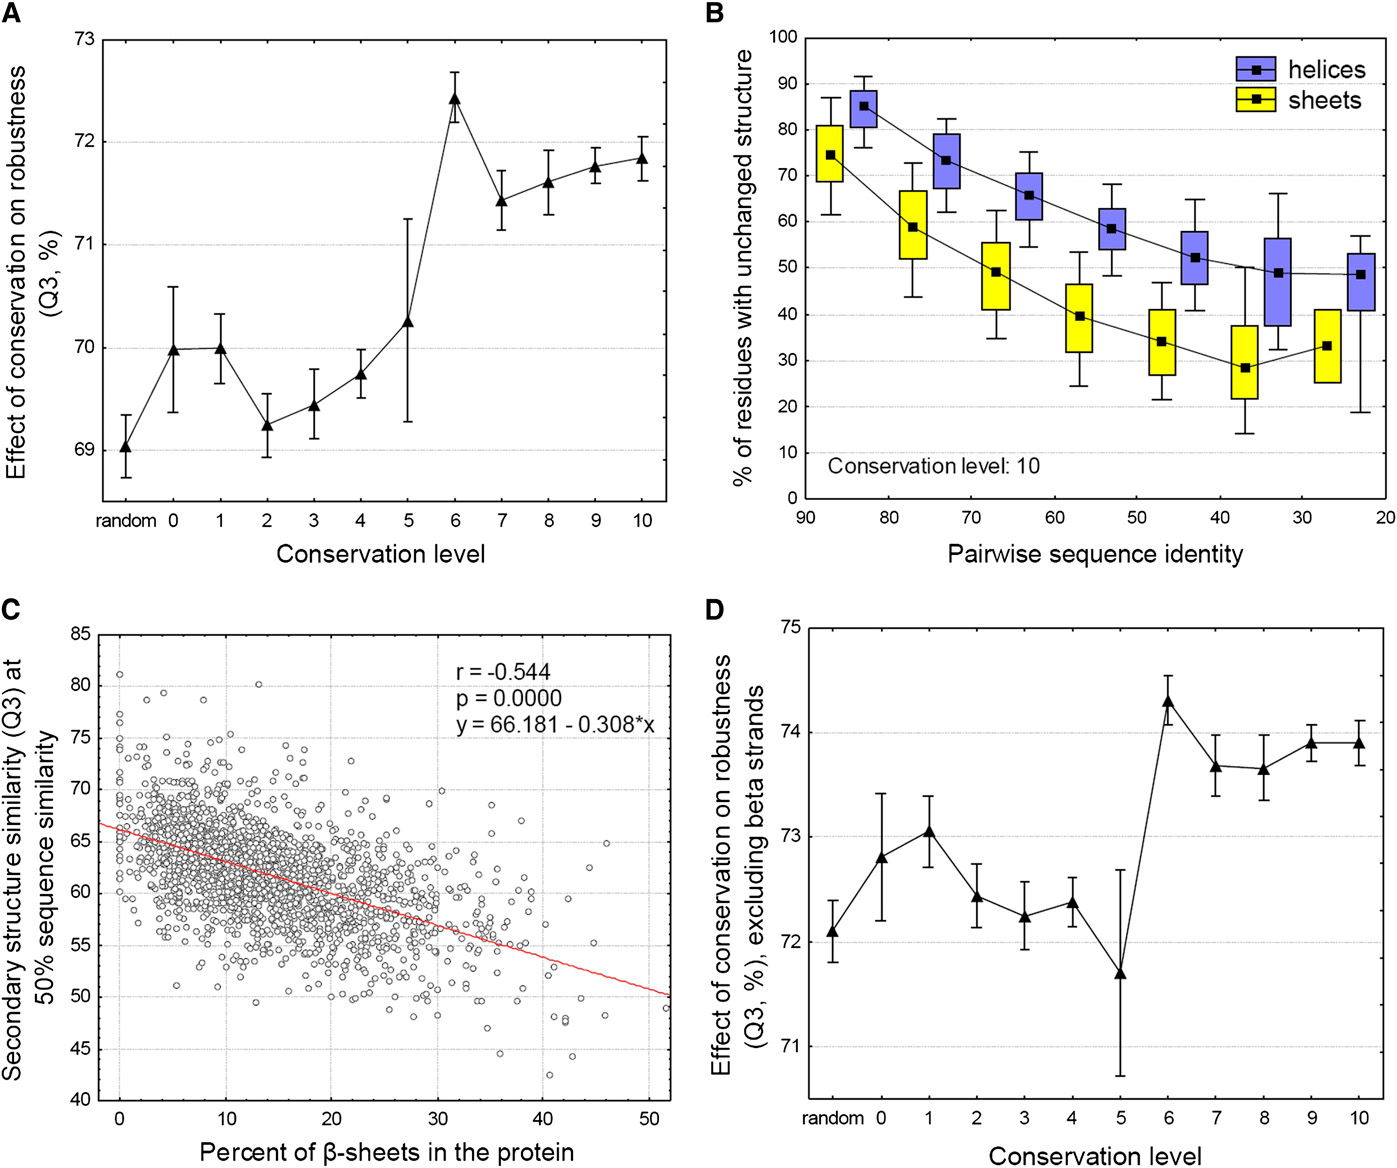
\includegraphics[scale=0.2]{abrusan-fig7} \caption{Abrusan
            (2013) protein robustness trends} \end{figure}

    \subsubsection{Deacrease in hydropathicity}

        Falls sharply in youngest strata, then seemingly steady
        \cite{carvunis_proto-genes_2012}

        POFs are more hydrophylic than PDFs \cite{gollery_what_2006}.

    \subsubsection{Number of transmembrane regions}

        Falls sharply in youngest strata, then seemingly steady
        \cite{carvunis_proto-genes_2012}
        

    \subsubsection{Folds}

        An exhaustive prediction of whole proteome folds using SEG-HCA. Special
        emphasis given to structural orphan domains \cite{faure_comprehensive_2013}.

\subsection{Gene properties} \subsubsection{Increase in GC content}
\subsubsection{Increase in exons count}

        Some report de novos seldom have introns (1/{60} in humans
        \cite{wu_novo_2011}). Others report common introns in de novos (5/{13}
        in Plasmodium \cite{yang_novo_2011}), 5/{69} in mouse and 4/{6} in rat
        \cite{murphy_novo_2012}).


    \subsubsection{Steady exon length}

        Steady except for increase in youngest
        \cite{neme_phylogenetic_2013}

    \subsubsection{Increase in codon usage deviation from random}

        Carvunis \cite{carvunis_proto-genes_2012}

    \subsubsection{Decrease in overlap with other genes}

        Orphan genes tend to overlap mature genes. 51/69 mouse and 3/6 rat
        de novo genes \cite{murphy_novo_2012}.

        This tendency could be the result of rising genes exploiting the
        transcribed state of their elders, or it could be an artefact of
        the superior annotation and knowledge of synteny in the vicinity of
        known genes.

        ``Another possibility, however, is that the common features are
        merely due to ascertainment biases resulting from the methods that
        are used to detect the de novo genes. We require relatively well-
        conserved synteny and identifiable and alignable homologous
        sequence between species in order to provide positive evidence of
        the absence of the gene from other lineages. Short genes that
        overlap with conserved genes are more likely to satisfy these
        criteria'' \cite[pp. 8]{murphy_novo_2012}.

        Neme observed the youngest genes often have relatively long
        promoters and are associated with bidirectional promoters
        \cite{neme_phylogenetic_2013}

    \subsubsection{GC content}

        In insects, higher GC content in ant-specific genes
        \cite{wissler_mechanisms_2013}


\subsection{Regulatory and properties}

  \subsubsection{Dosage dependence}

    Older biochemical pathways are more likely to be dosage-dependent than
    plant-specific pathways \cite{shi_genome-wide_2015}.

  \subsubsection{Integration into regulatory networks}

    Fast in yeast \cite{abrusan_integration_2013}

    \begin{figure}[h!] \centering
        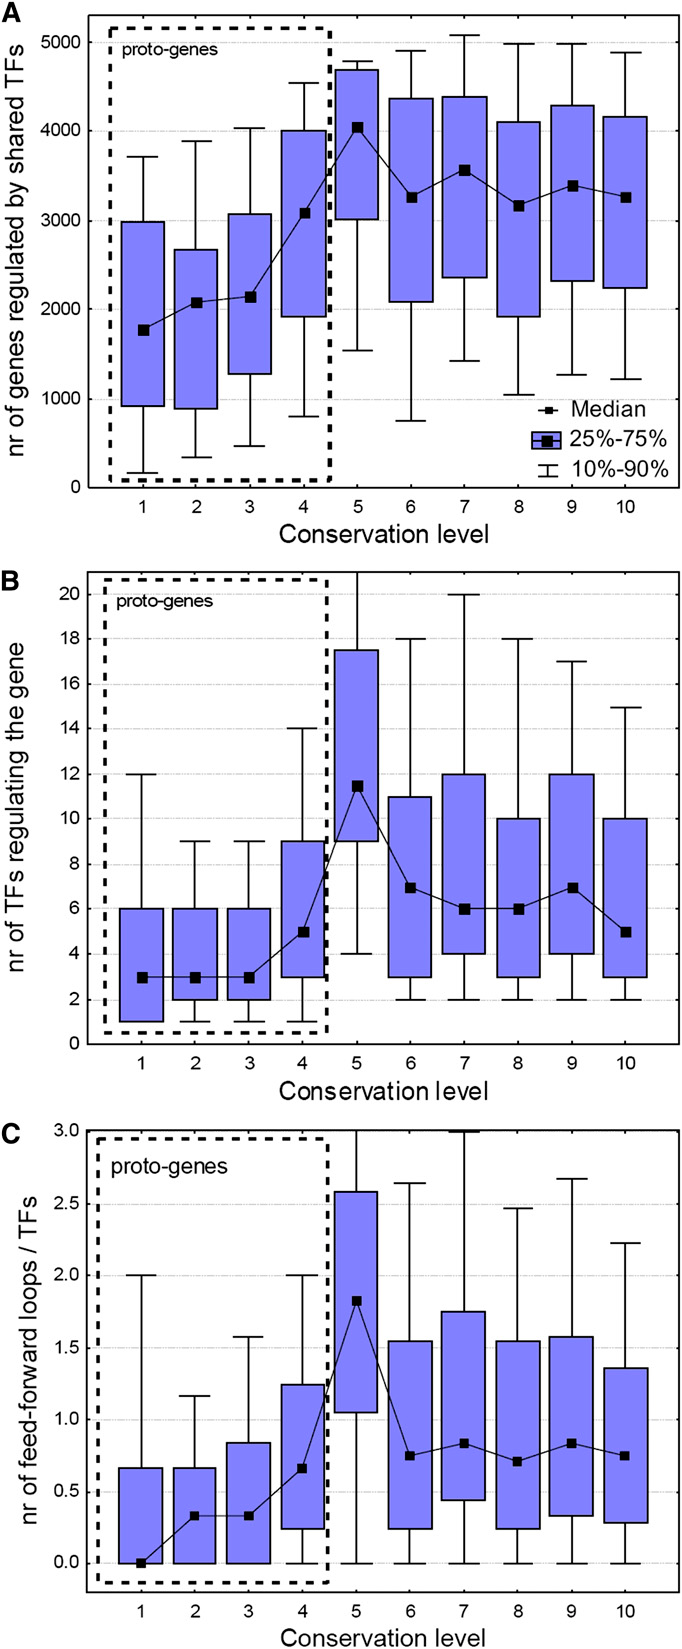
\includegraphics[scale=0.2]{abrusan-fig2} \caption{Abrusan
        (2013) regulatory trends} \end{figure} \FloatBarrier

    Young novel and duplicate genes integrate into networks differently
    \cite{capra_novel_2010}. Duplicate genes tend to modify old functions
    (unsurprisingly) while novel genes are more novel.

  \subsubsection{Localization}
              
    Localized in testes [cite], immune system [cite], and human
    brain \cite{li_human-specific_2010} in animals.
    Embryological localization across kingdoms [cite].  De novo
    genes highly expressed in human cerebral cortex
    \cite{wu_novo_2011}

  \subsubsection{Increase in expression}

    \begin{figure}[h!] \centering
        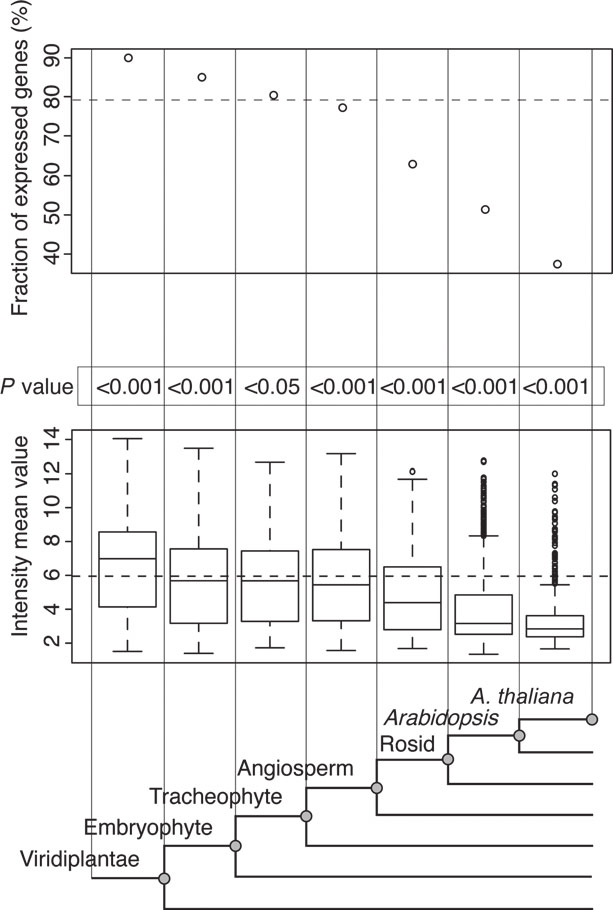
\includegraphics[scale=0.3]{guo_2012-fig5} \caption{ Guo (2013)
            Expression rate in Arabidopsis thaliana
            \cite{guo_gene_2013} } \end{figure} \FloatBarrier

    Somewhat erratic, but steady and highly significant, increase in
    expression in yeast \cite{carvunis_proto-genes_2012}.

\subsection{Evolutionary}

  \subsubsection{What factors affect evolutionary rate?}

    Mukherjee et al. performed an indepth regression analysis of the factors
    contributing to evolutionary rate in \textit{Leishmania major}
    \cite{mukherjee_elucidating_2015}. They found disorder content > Nc > CAI >
    protein hydrophilicity > gene expres- sion level > gene age > protein
    length. Although this is probably not generalizeable beyong \textit{L.
    magor}.
    

    \subsubsection{Increase in functionality?}
                
        Never as enzymes (true?). MDF1 in yeast regulates a mating pathway
        (decide between sexual and asexual reproduction in varying
        conditions) \cite{li_novo_2010}.

        Of 75 mouse and rat de novo genes, none have known domains or
        functional motifs \cite{murphy_novo_2012}.

    \subsubsection{Selective paradigm}

        \begin{figure}[h!] \centering
            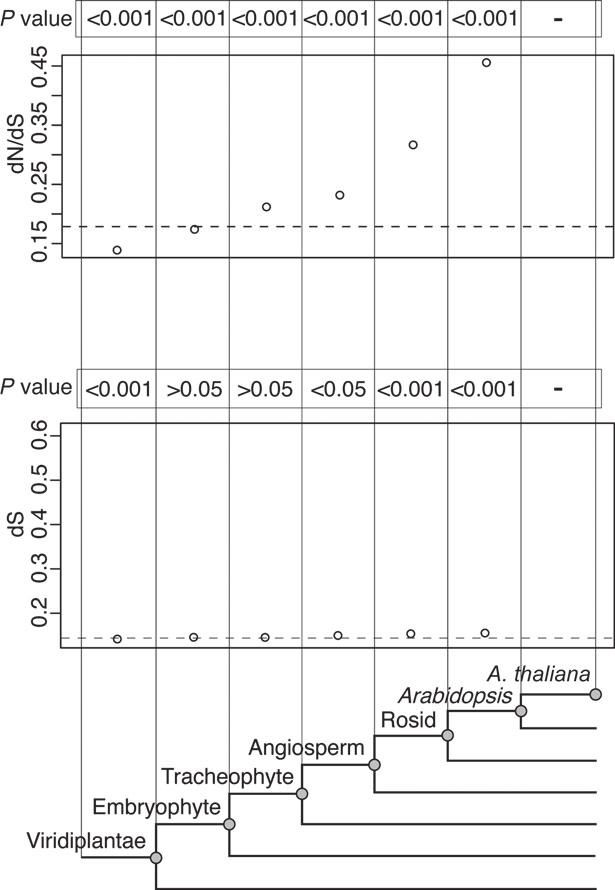
\includegraphics[scale=0.3]{guo_2012-fig6} \caption{ Guo (2012)
                dN/dS (non-synonymous / synonymous) mutation rate in
                Arabidopsis thaliana \cite{guo_gene_2013} } \end{figure}

        Also in Carvunis (see key papers fig. 3) strong purifying selection
        positive trend with age \cite{carvunis_proto-genes_2012}

        \begin{figure}[h!] \centering
            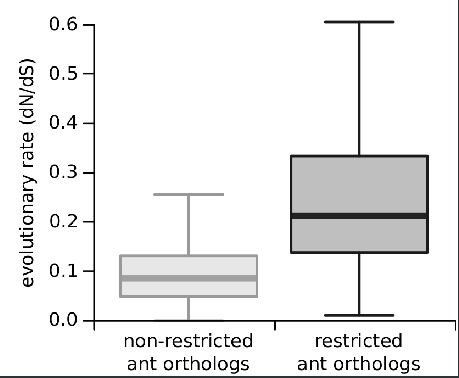
\includegraphics[scale=0.3]{wissler_insect_2013-supfig6c}
            \caption{ Wissler (2013) dN/dS in ants
                \cite{wissler_mechanisms_2013} } \end{figure}

        In corrals orphans are more likely to be under positive selection
        than non-orphans \cite{voolstra_rapid_2011}

        \begin{figure}[h!] \centering
            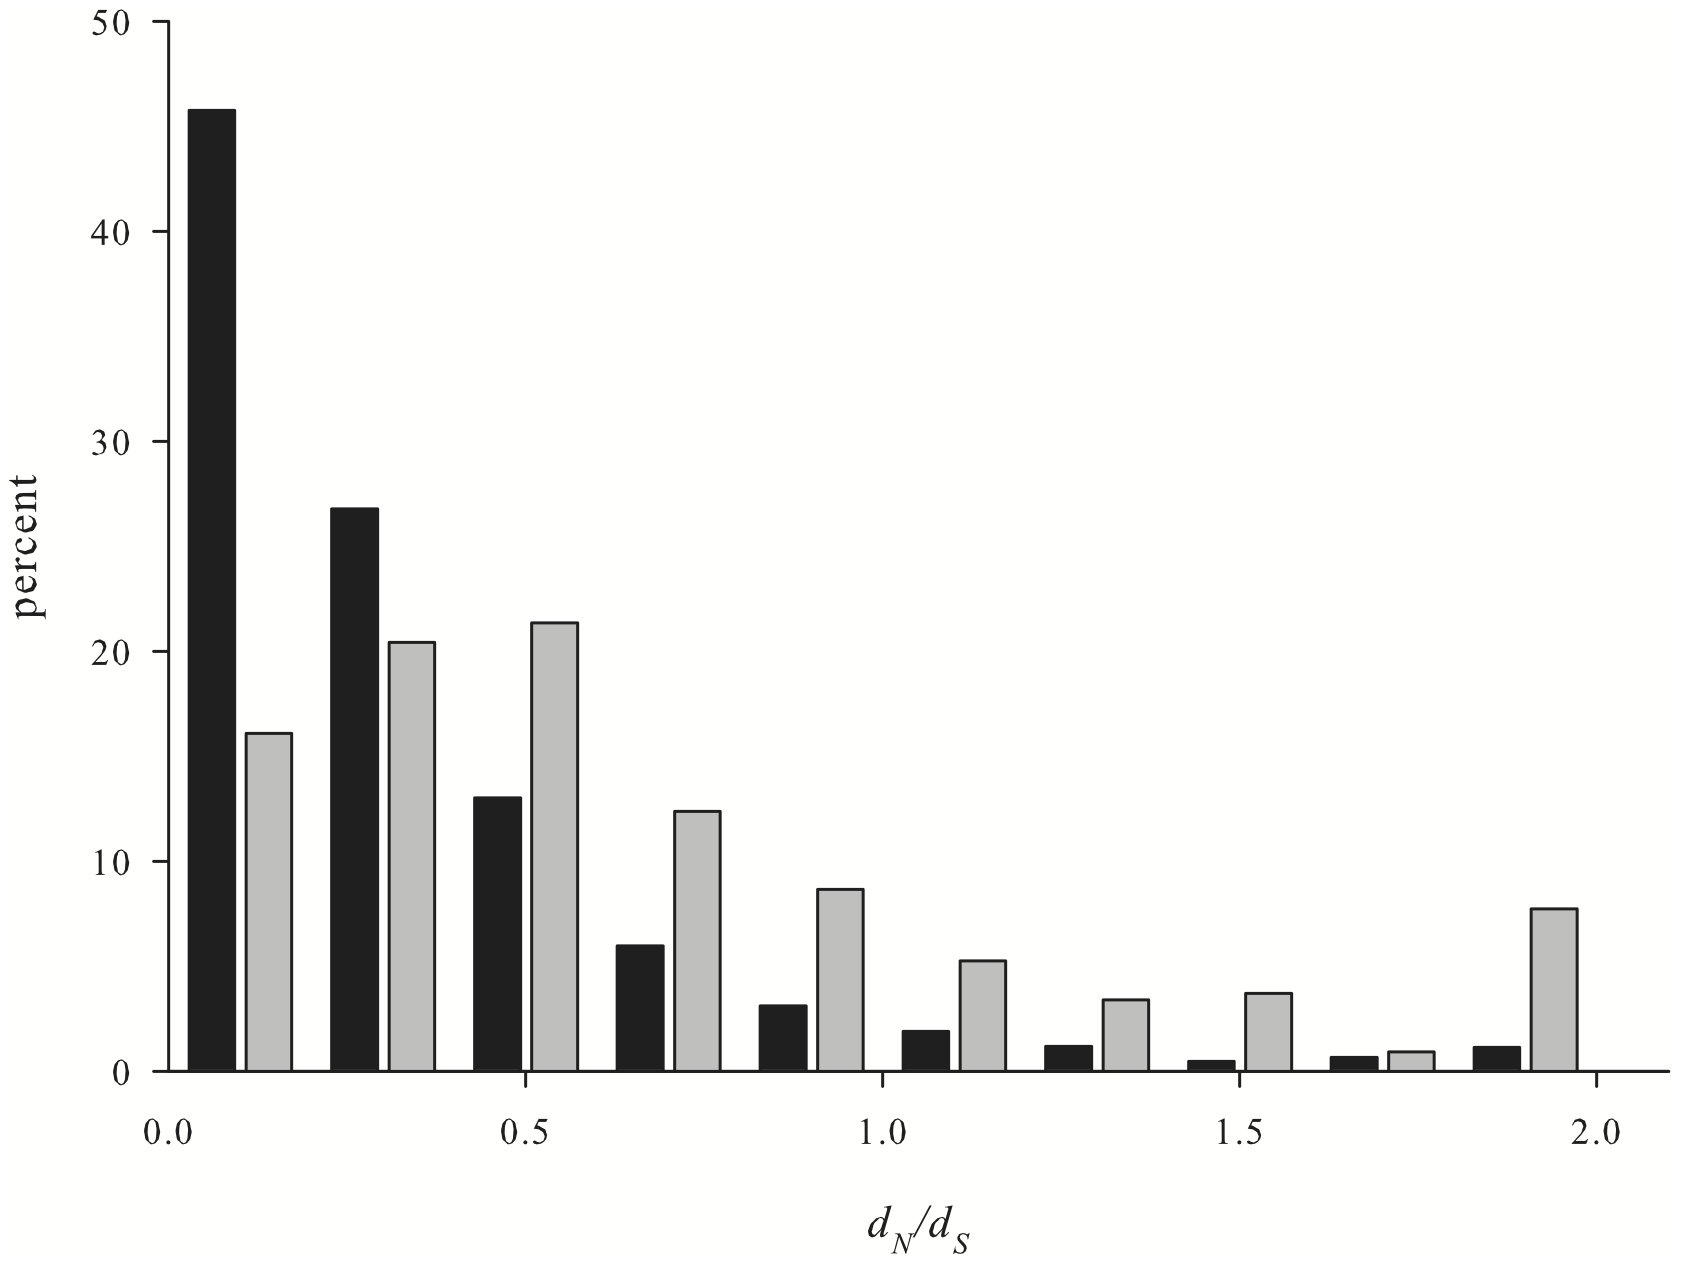
\includegraphics[scale=0.3]{voolstram_coral_2011-fig1}
            \caption{ Voolstram (2011) Corals, (black conserved, grey
                lineage-specific) \cite{voolstra_rapid_2011} } \end{figure}



        \FloatBarrier

    \subsubsection{Rise in essentiality}

        Relatively fast, youngest genes not usually essential
        \cite{abrusan_integration_2013}

        In Drosophila there is no difference in essentiality
        \cite{chen_new_2010}. 

        In mice, young genes are less likely to be essential
        \cite{chen_younger_2012}. Duplicates are less likely to be essential
        than singlets. It is important in any study of essentiality to consider
        this.

        \begin{figure}[h!]
            \centering
            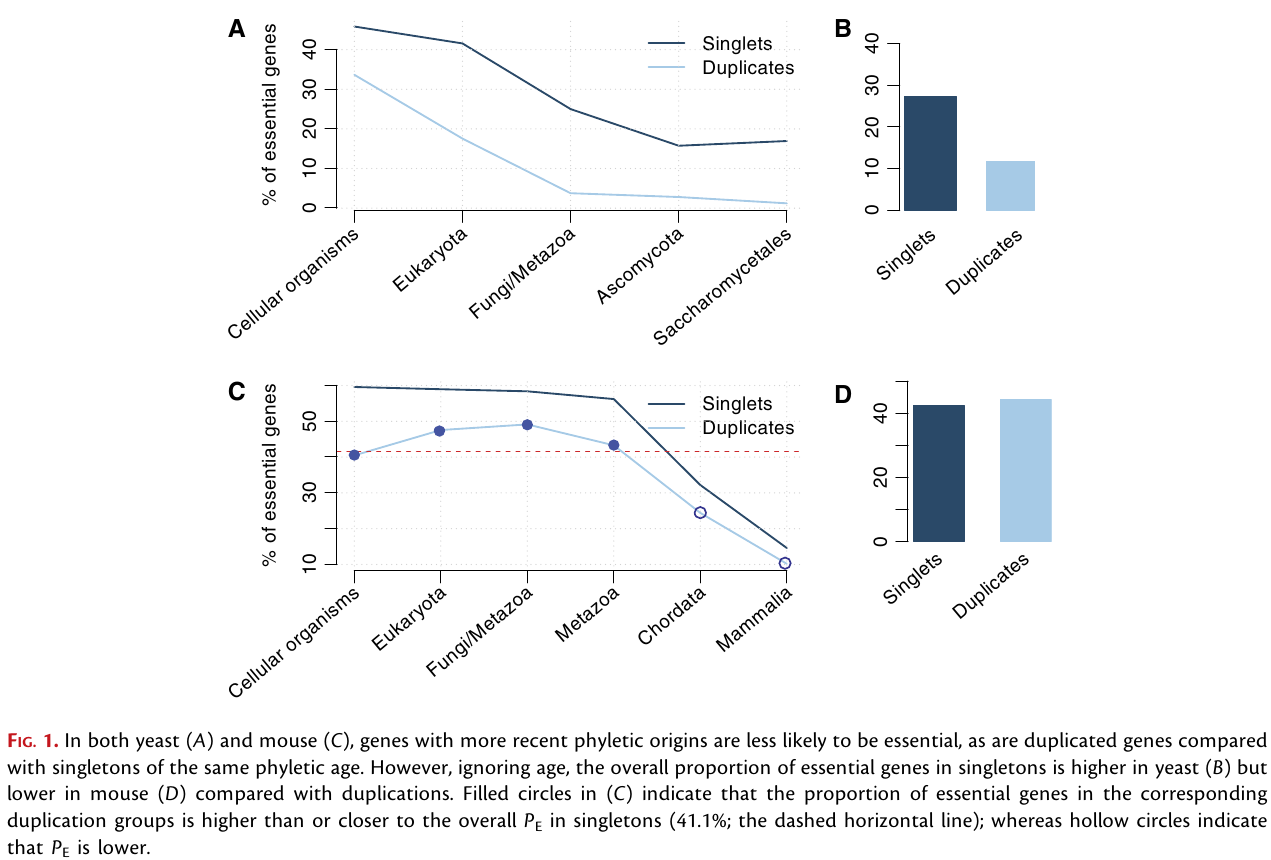
\includegraphics[width=0.9\textwidth]{chen-essential-2012-fig1}
            \caption{Chen (2012) fig1 \cite{chen_younger_2012}}
        \end{figure}

        \begin{figure}[h!] \centering
            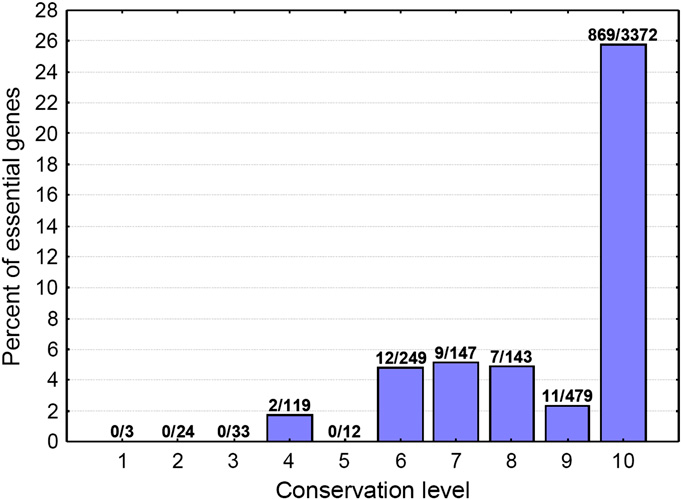
\includegraphics[scale=0.2]{abrusan-fig3}
            \caption{Abrusan (2013) essentiality trends}
        \end{figure}
        \FloatBarrier


\subsection{Network} \subsubsection{Increase in protein-protein
interactions}

        This is a gradual but steady process, much slower than rise in
        regulatory connectedness \cite{abrusan_integration_2013}. Abrusan
        reports a nearly monotonic increase in median of ~1 to ~20 across
        the strata.

        Of 14 plant species, no species-specific gene was a protein-protein
        hub (top 10\%) \cite{ye_evolutionary_2013}.


        \begin{figure}[h!] \centering
            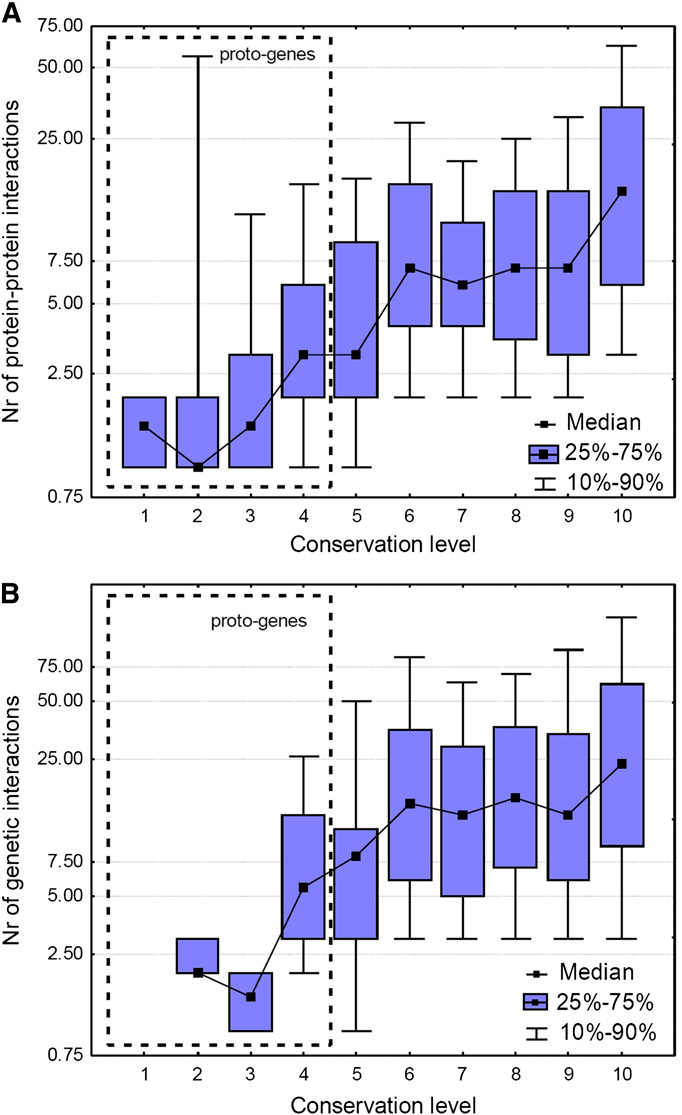
\includegraphics[scale=0.2]{abrusan-fig8} \caption{Abrusan
            (2013) protein-protein and genetic trends} \end{figure}

    \subsubsection{Increase in genetic interactions}

        Genetic interactions are the non-multiplicative fitness
        contributions of two genes.

        Abrusan reports a trend in genetic interactions that is nearly
        identical to the protein-protein interaction trend (not too
        surprising since the two are certainly dependent)
        \cite{abrusan_integration_2013}.

    \subsubsection{Broadening of expression}

        Primate specific genes are expressed in few tissues than ancient
        genes \cite{toll-riera_origin_2009}

        \begin{figure}[h!] \centering
            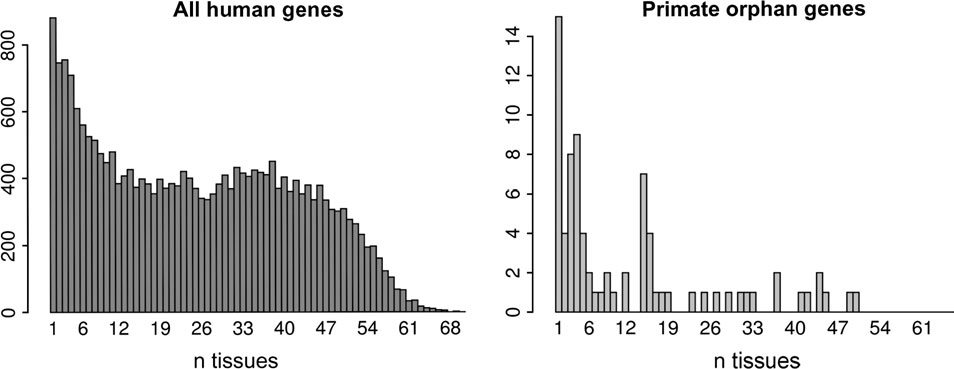
\includegraphics[width=16cm]{toll-riera_2009-fig1}
            \caption{Toll-riera \textit{et al.}} \end{figure} \FloatBarrier
